\def\latexktupreamblefile{scoring_manual.ktu_preamble}
\def\mytitle{scoringパッケージ}
\def\myauthor{山本}
\def\mydate{2019.6.25}
\def\latexxspacing{no}
\input{ltktu.tex}

\newcommand {\mycolor }{olive}

\section{scoringパッケージの概要}
\label{scoringパッケージの概要}

(この\texttt{readme.md}をtexでpdfにしたファイルが\texttt{test\slash scoring\_manual.pdf}にある)

採点作業の流れの中で以下のような作業をscoringパッケージはサポートする。

\begin{enumerate}
\item マークシートの採点

\begin{itemize}
\item マークシートの読取結果(csvファイル)を採点し、学籍番号と点数のcsvファイルを作成する

\end{itemize}

\item 統合

\begin{itemize}
\item マークシート以外の成績情報を統合する(例えば、宿題や筆記問題の採点結果などとの統合)

\end{itemize}

\item 分析

\begin{itemize}
\item 以下のような統計データを出力できるので、それを見て分析する

\item 各問題の正解割合, 評語(A+ABCD)の割合, 点数のヒストグラム, 基本統計, 学類別基本統計

\end{itemize}

\item 点数調整

\begin{itemize}
\item 点数調整を行って配点を調整する

\end{itemize}

\item Twinsアップロード用ファイルの作成

\begin{itemize}
\item 点数調整を行った最終結果をtwinsのアップロード用ファイルに統合する。

\end{itemize}

\end{enumerate}

\section{install}
\label{install}

installは以下の2つのファイルを正しい場所に配置すればよい。

\begin{itemize}
\item \texttt{src\slash scoring.py}: pythonのプログラム(モジュール)なので、pythonのライブラリパスが
通っているところにコピーする。

\item \texttt{bin\slash score}: scoringパッケージを呼び出すbashシェルなので、\texttt{PATH}が通っているところにコピーする。
scoringパッケージのすべての機能はこの\texttt{score}コマンドを通して提供される。

\end{itemize}

\texttt{make install}で配置したい場合は\texttt{Makefile}の中の以下の2つの変数を
正しくセットしてから、\texttt{make install}する。
\begin{tcolorbox}[enhanced jigsaw,breakable,colframe=\mycolor ,colback=white,colbacktitle=\mycolor ,coltitle=white,fonttitle=\bfseries\sffamily]

\begin{verbatim}
pylib = scoring.pyを入れるディレクトリ(普通は$PYTHONPATH)
bindir = scoreコマンドを入れるディレクトリ($PATHのどれか)
\end{verbatim}

\end{tcolorbox}

前提条件は以下。

\begin{itemize}
\item python3.6以上

\item pythonのpandasモジュール

\end{itemize}

\section{scoreコマンドの使い方}
\label{scoreコマンドの使い方}

scoringパッケージのすべての機能は\texttt{score}コマンドを経由して
提供される。すべての成績データ(入力・出力・途中結果)は学籍番号を必ず含む
csvファイルで表現される。\texttt{score}コマンドは少なくとも1つのcsvファイルを扱うので、
1つのcsvファイルは必須引数である。基本的に出力は\texttt{stdout}にcsvの形式で
加工された成績が出力される。また、分析用の情報は\texttt{stderr}に出力される。
\begin{tcolorbox}[enhanced jigsaw,breakable,colframe=\mycolor ,colback=white,colbacktitle=\mycolor ,coltitle=white,fonttitle=\bfseries\sffamily,title=\texttt{\$ score -h}]

\begin{verbatim}
usage: score [-h] [-marksheet ref-filename desired-pscore] [-crate] [-join filename]
             [-twins] [-adjust x y xmax] [-abcd] [-statistics] [-distribution]
             [-gakuruistat gakurui-filename] [-nostdout] [-interval min max]
             [-outputfile filename]
             csvfilename
\end{verbatim}

\end{tcolorbox}
オプション名は区別が可能な限り短縮してよい。\texttt{-adjust}と\texttt{-abcd}以外は
すべて1文字で区別できる。

必須引数である\texttt{csvfilename}は次のように3種類に解釈される。

\begin{itemize}
\item \texttt{-marksheet}オプションが指定された場合

\begin{itemize}
\item マークシートの読取結果(学生の解答ファイル)とみなされる

\begin{itemize}
\item headerなし

\item 1列目が学籍番号(下7桁), 2列目以降はマークシートのマーク番号

\end{itemize}

\end{itemize}

\item \texttt{-twins}オプションが指定された場合

\begin{itemize}
\item twinsアップロード用csvファイルと見なされる

\begin{itemize}
\item headerあり(ただし、scoreコマンドは無視する: shift-jisのため)

\item 列は左から'科目番号`,'学籍番号`, `学期区分','学期評価', `総合評価'

\item twinsからダウンロードしたままのファイルでOK

\end{itemize}

\item 上記の\texttt{-marksheet}オプションと排他的である

\end{itemize}

\item 上記以外

\begin{itemize}
\item 採点途中結果のcsvファイル

\begin{itemize}
\item headerなし

\item 1列目が学籍番号(9桁), 2列目が点数

\end{itemize}

\end{itemize}

\end{itemize}

\texttt{score}コマンドの出力はtwinsアップロードファイルへのjoinの場合を除いて、
すべて「採点途中結果のcsvファイル(headerなしの1列目が学籍番号(9桁),2列目が点数)」である。

以下では、作業の種別毎にオプションを説明する。

\subsection{マークシート採点}
\label{マークシート採点}

\subsubsection{\texttt{score csvfilename -marksheet ref-filename desired-pscore ...}}
\label{scorecsvfilename-marksheetref-filenamedesired-pscore...}

\texttt{csvfilename}をマークシート読み取り結果として読み込み、採点を行う。
マークシートの正解を定義したファイル(\texttt{ref-filename})を引数として与える。
また、マークシートの満点(\texttt{desired-pscore})を与える。正解定義中の各問題のweightに
したがって各問題に配点する(配点は整数なので要求した満点と
少し違うこともありえる)。
\texttt{-twins}以外の全てのオプションを同時に使用可能。
チェック用として各学生・各問題ごとの正誤(正=1, 誤=0)のcsvファイルを以下の
名称で保存する。

\begin{itemize}
\item \texttt{csvfilename.marubatu}

\end{itemize}

マークシート採点のための正解定義は\ref{mksheet-ref}節参照。
学籍番号はすべて頭に\texttt{20}が付けられるので(\texttt{200000000}を足す)、
必ず下7桁になっている必要がある。

\subsubsection{\texttt{-crate}}
\label{-crate}

\texttt{-marksheet}オプションが指定されているときだけ有効なオプションで、
各小問毎の正解率、配点、問題タイプを\texttt{stderr}に出力する。

\subsection{統合}
\label{統合}

\subsubsection{\texttt{score csvfilename -join csvfilename2 ...}}
\label{scorecsvfilename-joincsvfilename2...}

必須ファイル\texttt{csvfilename}で指定されたデータ\floatfootnote{\texttt{-marksheet}オプションが指定されている場合は、採点結果に対して適用される。}に\texttt{csvfilename2}で
指定されるデータを統合する。統合は、keyとして学籍番号を用い、
\texttt{pandas}の\texttt{merge}関数を用いる。統合(join)方法は以下の2種類。

\begin{itemize}
\item \texttt{-twins}オプションが指定されている場合:

\begin{itemize}
\item twinsアップロードファイルへleft-joinを行う。

\begin{itemize}
\item twinsのファイルにない学生は取り除かれる

\item 取り除く学生の学籍番号はstderrに出力される

\end{itemize}

\end{itemize}

\item \texttt{-twins}オプションがない場合:

\begin{itemize}
\item outer-joinを行う

\begin{itemize}
\item 片方のデータにしかない学生も残る。

\item データがない方の学生の点数は0点

\end{itemize}

\end{itemize}

\end{itemize}

\texttt{-twins}オプションがある場合の出力はtwinsへのアップロード用の
ファイルとして出力される。

\begin{itemize}
\item headerがshift-jisでないといけないので\texttt{-output}オプションでファイルを指定する。

\begin{itemize}
\item 標準出力に出すとなぜかshift-jisにならない\frownie 

\end{itemize}

\item twinsデータの'総合評価'に数値が入っている場合はそれと\texttt{csvfilename2}の点数の合計が'総合評価'になる

\item twinsデータの'総合評価'が空の場合は\texttt{csvfilename2}の点数が'総合評価'になる

\end{itemize}

\texttt{-join}オプションの引数である\texttt{csvfilename2}のファイルの仕様は以下。

\begin{itemize}
\item headerなし

\item 1列目: 学籍番号

\item 2列目以降(いくつでもOK): 評価点

\begin{itemize}
\item 2列目以降の点数は合計される

\item 統合後に\texttt{csvfilename}と\texttt{csvfilename2}の点数は合計される

\end{itemize}

\end{itemize}

他のあらゆるオプションを同時使用可能。

\subsection{点数調整}
\label{点数調整}

点数調整は、マークシート採点後または統合後、あるいはどちらも指定されてない場合は
\texttt{csvfilename}で与えられた処理途中のデータに対して適用される。

\subsubsection{\texttt{-adjust x y xmax}}
\label{-adjustxyxmax}

素点xをyに線型に持ち上げる。xmax以上は素点のまま。
図\ref{fig:adjust}を参照。

\begin{figure}[htbp]
\centering
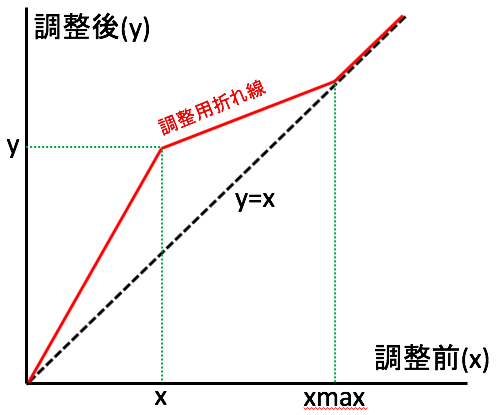
\includegraphics[keepaspectratio,width=5cm,height=0.75\textheight]{fig/adjust.png}
\caption{\texttt{-adjust x y xmax}の点数調整}
\label{fig:adjust}
\end{figure}

\subsubsection{\texttt{-interval min max}}
\label{-intervalminmax}

点数の最低点を\texttt{min}、最高点を\texttt{max}にする。

\subsection{分析}
\label{分析}

分析は点数調整後の成績に対して行われる(すなわち出力ファイルに対する
分析である)。以下のような種類(オプション名)があり、同時に指定できる。
出力はすべて\texttt{stderr}に出力される。

\begin{itemize}
\item \texttt{-distribution}: 点数分布のヒストグラム出力

\item \texttt{-abcd}: 標語(A+, A, B, C, D)の人数分布

\item \texttt{-statistics}: 平均, 標準偏差, 最高・最低点, 4分位点

\item \texttt{-gakuruistat gakurui-filename}: 学類毎の\texttt{statistics}

\begin{itemize}
\item 学類毎の学籍番号を定義したファイルを引数として与える

\item 定義ファイルの詳細は\ref{gakurui-info}節参照。

\end{itemize}

\end{itemize}

あらゆる他のオプションと同時併用できる。最終結果(すなわち出力データ)に対する
分析を行う。先に行われるのは、マークシート採点、統合、点数調整である。
いずれも指定されていない場合は、入力としての\texttt{csvfilename}がそのまま
分析対象となる。\texttt{-twins}オプションが指定されている場合は、
twinsへのアップロードファイルの分析が行われる。

点数調整と分析は同時に指定しながら調整するのが普通の使い方と思われる。

\subsection{その他}
\label{その他}

その他のオプションは以下。

\begin{itemize}
\item \texttt{-nostderr}: 標準出力に結果のcsvファイルを出力しない

\begin{itemize}
\item 調整時にこれを指定することが多い

\end{itemize}

\item \texttt{-output filename}: 結果を標準出力ではなくファイルに出力する

\begin{itemize}
\item twinsアップロード用ファイルはこのオプションで出力しないと
headerが正しくshift-jisで出力されない

\end{itemize}

\end{itemize}

\section{使用例}
\label{使用例}

\subsection{使用例1}
\label{使用例1}

ある科目の使用例。この科目では期末試験でマークシート問題と記述問題の
2種類の解答をしてもらった。また、宿題の点数が別に定義されている。

\begin{enumerate}
\item ファイルの準備

\begin{itemize}
\item マークシートの解答を\ensuremath{\sim}data\slash answer.csvに用意

\item 記述問題の採点結果と宿題の点数を\ensuremath{\sim}data\slash sup.csvに用意

\item twinsからアップロード用のファイルを\ensuremath{\sim}data\slash upload.csvに用意

\end{itemize}

\item マークシートの正解と学類別の学籍番号を定義したファイルを作成する

\begin{itemize}
\item 正解(と配点重み): reference.py

\item 学類学籍番号: gakurui\_id.py

\item どちらもpythonのlist形式の記述なので拡張子を\texttt{py}としているが、
気持ち悪ければ\texttt{txt}でもOK

\end{itemize}

\item マークシートの採点結果を点数化する関数totalscoreを定義。

\begin{itemize}
\item 今回は小問1問につき3点

\end{itemize}

\item マークシートの採点

\begin{itemize}
\item 小問の正解率と満点を80としたときの配点を保存

\begin{itemize}
\item \$ score \ensuremath{\sim}data\slash answer.csv -m reference.py 80 -c -n \&> crate.txt

\end{itemize}

\item マークシートだけの得点状況を分析

\begin{itemize}
\item \$ score \ensuremath{\sim}data\slash answer.csv -m reference.py 80 -s -d -abcd -n

\item 分析結果を残したい場合は最後に\texttt{\&> file.txt}を付ける

\end{itemize}

\item (マークシートだけの得点を少し調整する場合)

\begin{itemize}
\item \$ score \ensuremath{\sim}data\slash answer.csv -m reference.py 80 -d -adjust x y xmax -i min max -n

\item あるいは、正解の配点重みを変更してもよい

\end{itemize}

\item 結果を書き出す

\begin{itemize}
\item \$ score \ensuremath{\sim}data\slash answer.csv -m reference.py -adjust x y xmax > mksheet.csv

\end{itemize}

\end{itemize}

\item \textsubscript{data}\slash sup.csvを統合

\begin{itemize}
\item 統合する

\begin{itemize}
\item \$ score mksheet.csv -j \ensuremath{\sim}data\slash sup.csv > mksheet\_sup.csv

\end{itemize}

\item 得点調整を行う

\begin{itemize}
\item \$ score mksheet\_sup.csv -abcd -d -adjust x y xmax -n

\item (最低・最高点が{[0,100]}をはみ出す場合は\texttt{-i 0 100}を加える)

\end{itemize}

\item 結果を書き出す

\begin{itemize}
\item \$ score mksheet\_sup.csv -abcd -d -adjust x y xmax > mksheet\_sup\_adjust.csv

\end{itemize}

\item (上記の3つは同時に行うこともできる)

\begin{itemize}
\item \$ score mksheet.csv -j \ensuremath{\sim}data\slash sup.csv -abcd -d -adjust x y xmax > mksheet\_sup\_adjust.csv

\end{itemize}

\end{itemize}

\item twinsのアップロードファイルを作成

\begin{itemize}
\item \$ score \ensuremath{\sim}data\slash upload.csv -t -j mksheet\_sup\_adjust.csv -d > twins\_upload.csv

\item (最低・最高点が{[0,100]}をはみ出す場合は\texttt{-i 0 100}を加える)

\end{itemize}

\item 特別処理が必要な学生に対してtwins\_upload.csvを直接修正

\item 最終結果に対する分析結果を保存

\begin{itemize}
\item \$ score twins\_upload.csv -t -s -g gakurui\_id.py -d -abcd -n \&> result\_analysis.txt

\end{itemize}

\end{enumerate}

\subsection{使用例2}
\label{使用例2}

\texttt{test}ディレクトリ以下に簡単なデータが準備してある。
準備されているデータは例として参考にしてください。
\texttt{test}ディクレトリで\texttt{auto.sh}を起動すると使用例1の簡単化された手続きが実行される。
結果の例が\texttt{test\slash test-ref}ディレクトリ以下にあるので正しく動作しているかを確認のためにも使える。

\section{付録}
\label{付録}

\subsection{準備作業}
\label{準備作業}

必要な準備作業を以下にまとめる。

\subsubsection{マークシート読み取り}
\label{マークシート読み取り}

学類所有のマークシート読み取り装置を使って読み取る。
前提としているマークシートは以下。

\begin{itemize}
\item 教育ソフトウェア社の「総合カード053」(型番: C053)

\begin{itemize}
\item 学生番号欄: 7桁(なので、学籍番号下7桁をマークさせる)

\item 解答欄: 「1--9,0」の0--9の数をマークできる列が50列

\begin{itemize}
\item 上から1,2,3,{\ldots},9,0の順

\end{itemize}

\end{itemize}

\end{itemize}
学籍番号のマークをミスる学生がいるので手で修正(2019年度のある科目では、
320人中2人の学生がおかしな番号を入れていた)。
解答欄は修正しない。
結果として、1列目が学籍番号(下7桁)、2列目以降がマークシートの各列の解答番号と
なっているcsvファイルができればよい。

\paragraph{マークシート読取手順}
\label{マークシート読取手順}

以下のようにしてマークシートの解答をcsvファイルにする。

\begin{itemize}
\item 学類のマークシート読取装置と専用ノートパソコンを接続・起動

\item 「MarkView」というソフトを起動

\item 「シート読取り」を選択

\item レイアウト切り替え(総合053とかなんとかのレイアウトにする)

\item ファイル\Pisymbol{psy}{"AE}読取りデータ保存先の変更

\begin{itemize}
\item これでファイルが初期化されるみたい

\end{itemize}

\item 読取ボタン?を押す(累積される)

\begin{itemize}
\item 明示的なsave命令はない。自動で保存される。

\end{itemize}

\item ソフトを終了

\end{itemize}

\subsubsection{履修者名簿}
\label{履修者名簿}

成績アップロード用の履修者名簿をtwinsからダウンロード。
処理の最後にこのファイルに成績を統合する。
headerがshift-jisであるが、そのままでよい(scoringパッケージは
headerを読み飛ばす)。アップロードファイルを出力する場合は
shift-jisのheaderを\texttt{score}コマンドが付ける。

\subsubsection{正解の定義}
\label{正解の定義}

マークシート読み取り結果に対する正解を定義するファイルを
作成する必要がある。以下の種類の解答に対応。

\begin{itemize}
\item \texttt{S}: 選択肢から1つ選択

\item \texttt{SS}: 選択肢から1つ選択の連続

\item \texttt{MS}: 選択肢から複数選択(順不同)

\item \texttt{Num}: 数値。複数桁もOK

\end{itemize}
それぞれの種類について、マークシートの位置と正解を定義。
配点重みは指定しなければdefaultの100(\%)が各小問に設定される。
配点重みを調整したい場合は100(\%)を基準に上下する割合を指定する。
詳しくは\ref{mksheet-ref}節を参照。

\subsubsection{学類学生番号情報}
\label{学類学生番号情報}

学類毎の成績統計を出す場合は、学類毎の学籍番号を定義したファイルが必要。
学籍番号の範囲指定と個別指定ができる。詳しくは\ref{gakurui-info}節参照。

\subsection{マークシートの正解定義}
\label{mksheet-ref}

マークシート問題の正解定義はpythonのlist形式のファイルを作成し、
ファイル名を指定する。リストの要素が各問題の定義である。各問題は
次のような4種類である。以下の「列番号」とはマークシートの列の位置である(1から50)。

\begin{itemize}
\item \texttt{S}: 選択問題

\begin{itemize}
\item Format: {[S, 列番号, 正解 (, 配点重み)]}

\end{itemize}

\item \texttt{SS}: 選択問題の連続

\begin{itemize}
\item Format: {[S, {[列番号start, 列番号end]}, {[正解1, 正解2, {\ldots}]} (, 配点重み)]}

\begin{itemize}
\item 列番号startから列番号endまでの連続した列番号に対して、正解1,2,{\ldots}を正解とする。

\end{itemize}

\item 各列番号は独立の小問と見なされる

\begin{itemize}
\item 配点重みは各小問にそのまま適用される(小問数で割ったりしない)

\end{itemize}

\end{itemize}

\item \texttt{MS}: 複数選択問題

\begin{itemize}
\item Format: {[MS, {[列番号1, 列番号2, {\ldots}]}, {[正解1, 正解2, {\ldots}]} (, 配点重み)]}

\begin{itemize}
\item 正解は順不同

\item 解答に同じ答えがある場合は1つしか正解としない

\end{itemize}

\item \emph{正解}の数だけ小問があるとみなす

\begin{itemize}
\item 配点重みは各小問についてそのまま適用される(小問数で割ったりしない)

\end{itemize}

\item 列番号の数と正解の数は一致しなくてもよい(\emph{正解}の数だけ小問が定義される)。

\begin{itemize}
\item 選択する正解の数を指定しない場合(多めに列番号を指定しておく)

\item 正解の方が列数より多い場合もありえる

\end{itemize}

\end{itemize}

\item \texttt{Num}: 数値問題

\begin{itemize}
\item Format: {[Num, {[列番号1, 列番号2, {\ldots}]}, {[正解1, 正解2, {\ldots}]} (, 配点重み)]}

\begin{itemize}
\item 正解の順番も一致しないと誤りと判断

\end{itemize}

\item 数値全体がすべて一致してこの小問1問正解とみなす

\end{itemize}

\end{itemize}
「配点重み」は省略されている場合\texttt{100}となり、\texttt{100}でない場合は\texttt{100}を基準
とした割合で指定する。

例えば以下の通り。4つ目の\texttt{MS}問題だけ各小問を配点重み\texttt{50}の割合いとしている。
他の(小)問の配点重みは指定していないのでdefaultの\texttt{100}となる。
実際の配点は指定した満点に応じた割合で決定される(整数化するため指定した
満点と少し誤差が出ることがある)。
\begin{tcolorbox}[enhanced jigsaw,breakable,colframe=\mycolor ,colback=white,colbacktitle=\mycolor ,coltitle=white,fonttitle=\bfseries\sffamily,title=正解定義ファイルの例]

\begin{verbatim}
[
    [S, 1, 1],
    [S, 2, 3],
    [S, 3, 6],
    [MS, [4,5,6], [2,4,5], 50],
    [Num, [7,8,9,10], [1,0,4,0]],
    [Num, [11,12,13], [5,4,0]]
]
\end{verbatim}

\end{tcolorbox}

\subsection{学類学籍番号情報}
\label{gakurui-info}

学類ごとの学籍番号の定義は、pythonのlist形式のファイルを作成し、
それを読み込ませる必要がある。
リストの各要素が各学類の学籍番号情報である。以下で定義される。
\begin{tcolorbox}[enhanced jigsaw,breakable,colframe=\mycolor ,colback=white,colbacktitle=\mycolor ,coltitle=white,fonttitle=\bfseries\sffamily]

\begin{verbatim}
学類学籍番号の定義ファイル = [ 学類情報1, 学類情報2, ...]
    学類情報i = [学類名の文字列, 範囲リスト, 個別リスト]
        範囲リスト = [範囲1, 範囲2, ...]
            範囲i = [start, end] : startからendまでの学籍番号
        個別リスト = [学籍番号1, 学籍番号2, ...]
            学籍番号i = 学籍番号を数値で
\end{verbatim}

\end{tcolorbox}
例えば以下の通り。
\begin{tcolorbox}[enhanced jigsaw,breakable,colframe=\mycolor ,colback=white,colbacktitle=\mycolor ,coltitle=white,fonttitle=\bfseries\sffamily,title=学類学籍番号情報定義]

\begin{verbatim}
[
    ['人文学類', [[210010250, 210010350], [209910111]],
    ['社会工学類', [[210022222, 210022333]], []],
    ['情報科学類', [[210044444, 210044555], [210055555, 2100555560]], []],
    ['情報メディア創成学類', [[210066000, 210066055]], [209911111, 209822222]],
    ['知識情報・図書館学類', [[210077000, 210077100], [220088888, 220088999]], []],
] 
\end{verbatim}

\end{tcolorbox}

\hfill  以上

\end{document}
